\documentclass{article}

\usepackage{lmodern}
\usepackage[UTF8]{ctex}% 中文语言包
\usepackage{amsmath}
\usepackage{booktabs}% 引入三线表宏包
\usepackage{indentfirst}% 使用indentfirst宏包
\setlength{\parindent}{2em}% 设置首行缩进距离
\usepackage{graphicx}% 插入图片宏包
\usepackage{float}% 图片错位解决

\begin{document}
    

\section{摘要}

vchain一个区块链系统能保证查询完整性。由于现存的部分解决方案要么存在丢失查询完整性的问题,要么就需要用户保存大量的区块链数据库的复制。但是使用一种新的可验证的查询处理框架,vchain允许一种轻量级用户去验证来自潜在不信任的服务提供商的查询结果



\section{引言}

区块链能使互不信任各方在没有权威中心的情况下,维护一个共同交易账本。从数据库的角度看,一个区块链能被看成是一个存储着大量带时间戳的数据记录集合的数据库。尽管区块链数据库已经开发了类似SQL的搜索引擎,但是现有的解决方案依赖于一个中心,中心则基于区块链数据库的物化视图,能忠实地执行用户的查询。

在不信任的环境中,这些解决方案存在失去查询完整性的风险,尤其是当中心服务器是恶意的或者是脆弱的时候。或者说,用户可以在本地保存一份数据库的复制,但是这对于普通的用户是不现实的。

为了解决这个问题,就提出来vchain,一个应用可验证的查询框架来保证查询完整性的区块链系统。其结构如下图所示:

\begin{figure}[H]
    \centering
    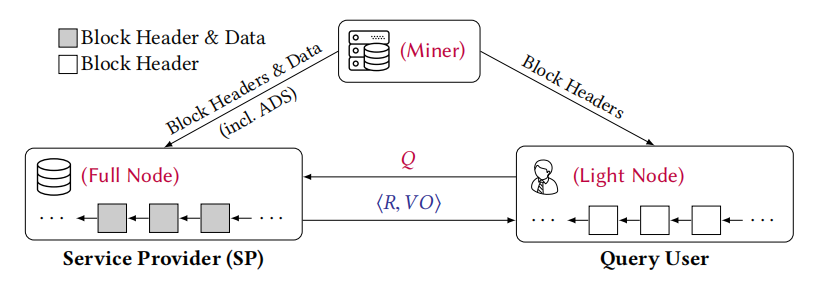
\includegraphics[width = 8cm]{img/vchain-1.png}
    \caption{vChain的系统模型}
\end{figure}

一个查询用户仅需要保存区块链头部作为一个轻节点;查询则外包给区块链网络中的一个全节点,作为服务提供者(SP)。尽管SP可能不受信任,但是查询用户可以通过检查其他验证对象VO来验证结果。

VO是由SP通过嵌入在块头中精心设计的身份验证数据结构(ADS)来计算的。为了进一步提高性能,还开发了几种基于索引的批处理验证技术,

\section{技术背景}

元组$<t_i,V_i,W_i>$表示存储在区块链数据库中的一个对象。

$t_i$时间戳

$V_i$一个或多个数值属性的多维向量

$W_i$ 是一个设置值属性

布尔范围的查询是如下形式:$q = <[t_s,t_e],[\alpha,\beta],\Upsilon >$

$[t_s,t_e]$ 针对该时间段的时间范围选择谓词

$[\alpha,\beta]$ 针对数值属性的多维范围选择谓词

$\Upsilon$ 是设置值属性的单调布尔函数

为了回应$q$,SP会返回所有对象,如$\{o_i=<t_i,V_i,W_i>|t_i \in[t_s,t_e] \wedge V_i \in [\alpha,\beta] \wedge \Upsilon(W_i) = 1\}$


\section{ADS生成与查询过程}

一种简单的方式是使用Merkle哈希树(MHT)作为ADS,并医用传统的基于MHT的身份验证。但是有三个缺点:

\begin{enumerate}
    \item MHT只支持构建Merkle树的查询键,为了支持涉及任意属性集的查询,需要为每个块构造一个指数级MHT
    \item MHT不能用于集合-值属性
    \item 不同块的MHT不能有效聚合,无法利用块间优化技术
\end{enumerate}

为了克服以上问题,提出了基于加密多集合累加器:

\begin{enumerate}
    \item 给定一个multiset $X$,能够计算一个累积值$acc(X)$,是一个防冲突的multiset的摘要
    \item 给定两个multiset $X_1$ $X_2$,且 $X_1 \cap X_2 = \emptyset $,可以计算出一个不相交的证明$\pi$
    \item 给定两个累加值 $acc(X_1)$,$acc(X_2)$,而且不相交的证明$\pi$可以验证$X_1 \cap X_2 = \emptyset $
    \item 给定两个累加值 $acc(X_1)$,$acc(X_2)$,则multiset$X_1+X_2$的累加值可以表示如下:$acc(X_1+X_2) = acc(X_1)+acc(X_2)$
\end{enumerate}

为了计算对象$o_i=<t_i,V_i,W_i>$的摘要,先将数值向量$V_i$转化成一组二进制前缀属性。

例如一个值4要被转换成$trans(4)=\{1*,10*,100\}$,其中$*$代表匹配计算的通配符

然后digest就通过集合值属性$W_i$和变换后的数值向量$trans(V_i)$进行累加得到:

$$
Digest_i = acc(W_i+trans(V_i))
$$

这个digest被用作ADS

给定一个数据对象和查询条件,那么只有两种结果:匹配或者不匹配。通过直接返回对象,第一种情况的可靠性可以轻易验证,因其完整性可以通过存储在块头中的hash验证

第二种情况就要使用对象的digest

一个以合取范式表示的bool函数可以被看做集合的列表。

例如,查询范围[0,6]相当于布尔函数$0*\vee 10* \vee 110 $。在转换后,一个范围查询能用与布尔查询相同的方式进行处理

\section{批验证}

对于每个查询,在查询的时间段内可能会存在多个要处理的对象。尽管可以逐个处理,但更好的方法是根据查询条件分批处理。为此,vChain提出了三种批验证技术

\subsection{块内索引}

如果两个对象的共享某个共同的属性值,则它们可能会由于存在相同的查询条件却不匹配查询。为了减少证明和验证开销,vChain构造了一个聚合块内对象的块内索引。

该索引是一种自下而上的方式构建的类似MHT的二进制树。对于每一个对象都会存在一个叶结点,然后递归合并两个最相似的树节点,直到根。对于每个非叶节点n,会被当做一个属性值的并集。

同时,对于两个相似的左右节点结点,存在$W_n = W_{n_l}\cup W_{n_r}$我们还要计算其digest作为acc($W_n$),以及它的hash值,最终的结果为

$$hash(hash(hash_{n_l}|hash_{n_r})|Digest_n)$$

使用块内索引,可以使用树节点及其相应的摘要来证明所有下方对象不匹配相同查询条件,从而提高查询性能。

\subsection{块间索引}

块间索引的工作方式类似于块内索引。不同之处在于,它用于跨多个块聚合对象。基于跳过列表,对于跳过块、跳过对象的聚合属性集以及相应的累加值求hash值,每个跳转包含他们的hash值。跳转中所有的对象都与相同的查询条件不匹配时,块间索引可以帮助提高查询性能。

\begin{figure}[H]
    \centering
    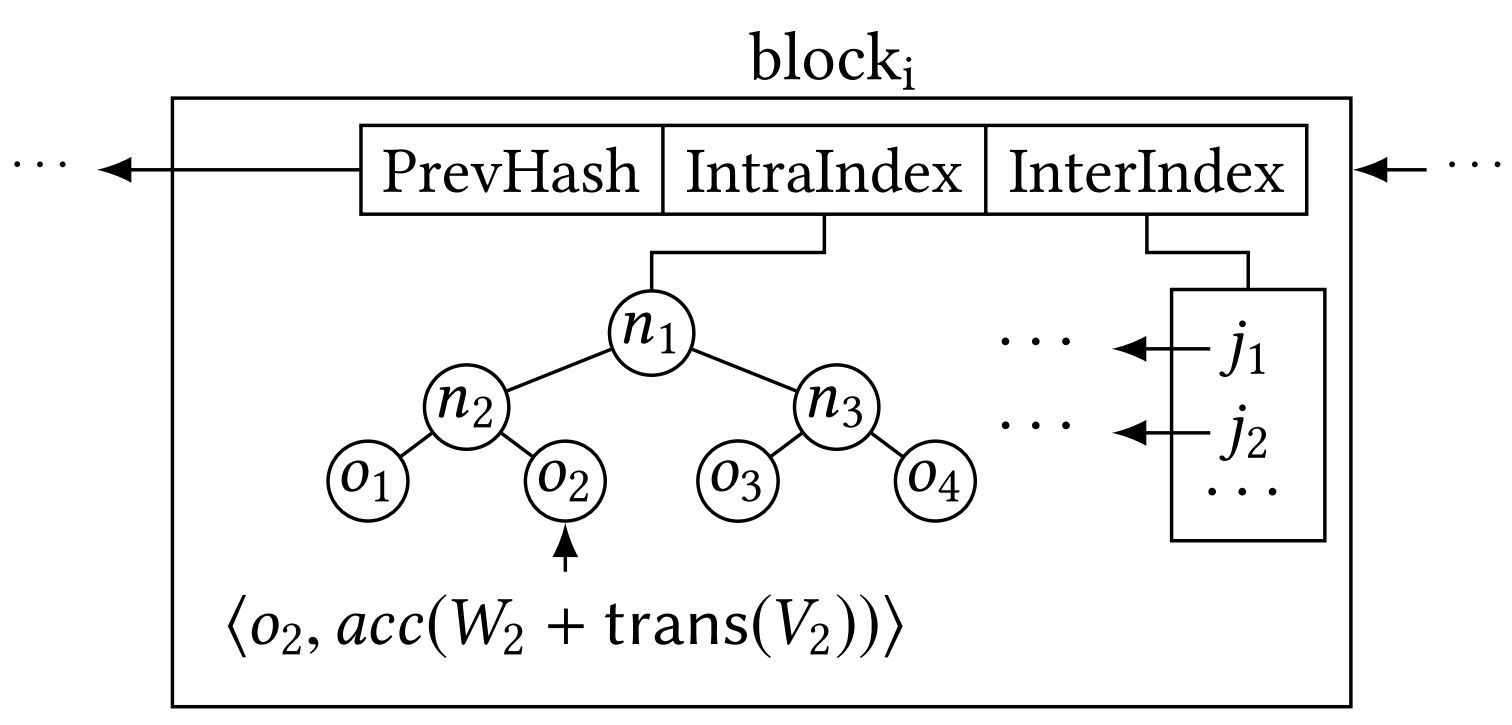
\includegraphics[width=12cm]{img/vchain-2.png}
    \caption{块内索引和块间索引}
\end{figure}

\subsection{在线批处理验证}

索引尝试将同一块或跨块的对象聚类,以最大限度的证明不匹配对象的效率。。然而在不同块甚至不同块的不同子树中索引的一些对象也可能共享相同的不同匹配原因。

\section{系统总览}

最底层是Exonum区块链框架,提供数据存储、P2P网络、区块链共识协议和区块链交易执行的基本功能。

中间层由几个低级模块组成。加密引擎提供计算加密hash函数,设置累加值和不相交证明的功能。使用了256位的BLAKE2b作为hash函数。

顶层则提供可验证的布尔范围查询的核心功能:

1. 矿工的ADS生成

2. SP查询处理

3. 用户的结果验证

\end{document}